\documentclass[twocolumn]{article}
\usepackage[margin=0.6in,columnsep=0.15in]{geometry}
\usepackage[utf8]{inputenc}
\usepackage{stix}
\usepackage[usenames,dvipsnames]{xcolor}
\usepackage[colorlinks,citecolor=Gray,urlcolor=Gray,linkcolor=Blue]{hyperref}
\usepackage[small]{titlesec}

\usepackage{authblk}
\renewcommand\Affilfont{\itshape\small} % chktex 6

\usepackage[normal]{caption}
\DeclareCaptionLabelSeparator{pipe}{ $|$ }
\captionsetup{labelsep=pipe}
\renewcommand{\captionfont}{\small}
\renewcommand{\captionlabelfont}{\bfseries}

\usepackage[sort&compress]{natbib}
\bibliographystyle{abbrvnat}
\renewcommand\cite{\citep}
\usepackage{doi}

\usepackage{graphicx}
\usepackage{mathtools}
\usepackage{booktabs}
\usepackage{tabularx}
\usepackage{tikz}

\title{\input{title.txt}}

\author[1,2]{Jan Hermann}
\author[2,*]{Alexandre Tkatchenko}
\affil[1]{Fritz-Haber-Institut der Max-Planck-Gesellschaft, Faradayweg 4--6, 14195 Berlin, Germany}
\affil[2]{Physics and Materials Science Research Unit, University of Luxembourg, 162A Avenue de la Faïencerie, L-1511 Luxembourg}

\date{}

\setcounter{secnumdepth}{0}

\begin{document}

\nocite{achemso-control}

\twocolumn[{
  \maketitle
  \vspace{-3em}
  \begin{center}
  \begin{minipage}{0.85\linewidth}
    \small
    \paragraph{Abstract}Short-range correlations in motion of electrons in matter are captured well by semilocal exchange--correlation (XC) functionals in density functional theory (DFT), but long-range correlations are neglected in such models and must be treated by van der Waals (vdW) dispersion methods.
Whereas the effective range of distances at which fluctuations are correlated is usually explicit in the vdW models, the complementary range of semilocal functionals can be observed only implicitly, requiring an introduction of empirical damping functions to couple the semilocal and nonlocal contributions to the XC energy.
We present a comprehensive study of the interplay between these short-range and long-range energy contributions in eight semilocal functionals (LDA, PBE, TPSS, SCAN, PBE0, B3LYP, SCAN0, M06-L) and three vdW models (MBD, D3, VV10) on noncovalently bonded organic dimers (S66), molecular crystals (X23), and supramolecular complexes (S12L), as well as on a series of graphene-flake dimers, covering a range of intermolecular distances (1.5--7\,\AA) and binding energies (0.5--130\,kcal/mol).
The binding-energy profiles of many of the DFT+vdW combinations differ both quantitatively and qualitatively, and some of the qualitative differences are independent of the choice of the vdW model, establishing them as intrinsic properties of the respective semilocal functionals.
We find that while the SCAN+vdW method yields a narrow range of binding energy errors, the effective range of SCAN depends on system size, and we link this behavior to the specific dependence of SCAN on the electron localization function $\alpha$ around $\alpha=1$.
Our study provides a systematic procedure to evaluate the consistency of semilocal XC functionals when paired with nonlocal vdW models, and leads us to conclude that nonempirical generalized-gradient and hybrid functionals are currently among the most balanced semilocal choices for vdW systems.

  \end{minipage}
  \end{center}
  \vspace{1em}
}]

\begingroup
\renewcommand\thefootnote{}\footnote{$^*$Email: alexandre.tkatchenko@uni.lu}%
\addtocounter{footnote}{-1}%
\endgroup

\section{Introduction}

In a true many-body electronic wave function, the motions of electrons are dynamically correlated across the entire range of inter-electronic distances.
A large part of this correlation is efficiently captured by various approximations to the Kohn--Sham density-functional theory (KS-DFT)~\cite{KohnPR65}, which established it as a basic tool in computational chemistry and condensed-matter physics.
But the standard density functionals are semi-local in space, resulting in electron correlation energy that decays exponentially with distance---as if the electrons were essentially uncorrelated at long range (except for the special case of slowly-varying electron density).
This leads to severe underestimation of van der Waals (vdW) dispersion interactions, which are mostly caused by long-range electron correlation.
As these interactions strongly contribute to properties of nearly all biological and modern synthetic materials, many models were developed that account specifically for the long-range correlation~\cite{DionPRL04,VydrovJCP10a,JohnsonJCP06,TkatchenkoPRL09,GrimmeJCP10,AmbrosettiJCP14} to augment the semi-local (or hybrid) density-functional calculations.
The range separation of electron correlation into short-range and long-range models can be in principle done formally~\cite{HermannCR17}, but insufficient knowledge about the ranges of different semi-local functionals prevents this in practice, having lead to various semi-empirical approaches.

The SCAN functional is a recent first-principles semi-local functional~\cite{SunPRL15} with great performance across a broad range of systems in chemistry and physics, in many cases reaching the accuracy of hybrid functionals at a fraction of their cost~\cite{SunNC16}.
It is still only semi-local, however, and does not describe long-range electron correlation, and hence vdW interactions.
On the other hand, the many-body dispersion (MBD) method is a general model of long-range electron correlation~\cite{TkatchenkoPRL12,AmbrosettiJCP14} that can be combined with any short-range correlation method, such as semi-local DFT or the density-functional tight-binding method.
The crossover regime, where a short-range description blends with the long-range MBD description, is controlled with a single range-separation parameter within the MBD model.
When trying to adjust this parameter for the SCAN functional---essentially estimating the correlation range of SCAN for vdW interactions---we observed that the optimal value depends significantly on the choice of the studied systems and the choice of the optimized quantity.
Since this is not the case for other density functionals such as PBE, we set out to study in general the range of electron correlation as described by different density functionals in vdW-bound systems.

\section{Background}

\paragraph{Density functionals: Short-range correlation models}

Some aspects of the ``tail'' behavior of semi-local density functionals in vdW systems are known, mostly from observations made on particular systems.
The Hartree--Fock (HF) model separates electron correlation into the exchange and ``pure'' correlation parts, the second of which is exclusively responsible for vdW attraction.
This does not translate well into exchange and correlation as approximated by semi-local density functionals in DFT, where the exchange part often contributes much more than the correlation part to the vdW attraction at equilibrium distances.
This behavior is caused by the implicit cancellation of errors between the two parts, and is reflected by the fact that most of the literature on this topic is concerned with exchange, not correlation functionals.
(See ref.\,\citenum{PengPRX16} for a more detailed discussion.)

Nearly all exchange energy functionals of the electron density, $n$, are constructed such that they are exact for the uniform electron gas, and are therefore of the form
\begin{equation}
  E_\mathrm x[n]=\int\mathrm d\mathbf rn(\mathbf r)\varepsilon^\text{unif}_\text x(n(\mathbf r))F_\mathrm x[n](\mathbf r)
  \label{eq:exchange-form}
\end{equation}
where the exchange energy density of a uniform electron gas, $\varepsilon^\text{unif}_\mathrm x(n)=-3k_\mathrm F(n)/4\pi$, $k_\mathrm F(n)(3\pi^2n)^{1/3}$, is multiplied with the so-called enhancement factor, $F_\mathrm x[n](\mathbf r)$, which goes to zero for a homogeneous density.
(This is also the reason why all such functionals describe the electron correlation energy completely in the uniform gas, including the long range part.
However, since this description is only local and effective, it does not transfer into inhomogeneous systems, which vdW-bound systems inherently are.)

The functionals studied in this work span first four rungs of the Jacob's ladder of density functionals.
The local density approximation (LDA, first rung) is defined by setting $F_\mathrm x[n]=1$~\cite{DiracMPCPS30}.
In a generalized gradient approximation (GGA, second rung), the enhancement factor depends locally on the dimensionless density gradient, $s[n]=\lvert\boldsymbol\nabla n\rvert/2k_\text F(n)n$, $F_\mathrm x(\mathbf r)=F^\text{GGA}_\mathrm x(s(\mathbf r))$, and it is the particular form of $F^\text{GGA}_\mathrm x(s)$ that distinguishes different GGAs.
Our study includes the GGA functional from Perdew, Burke, and Ernzerhof (PBE)~\cite{PerdewPRL96}.

The search for semi-local functionals with the appropriate correlation range has been done mostly within the space of GGAs and in the context of the vdW-DF non-local functional~\cite{DionPRL04,LeePRB10,MurrayJCTC09}, a long-range correlation method whose correlation range is not easily modified.
Several special-purpose functionals designed to combine well with long-range correlation models were developed, ranging from completely new constructions~\cite{PernalPRL09,WellendorffPRB12}, to recombinations of older forms~\cite{CooperPRB10,HamadaPRB14,BerlandPRB14}, to simple reparameterizations of standard functionals~\cite{ZhangPRL98,KlimesJPCM10,KlimesPRB11}.
(An ``ideal'' exchange functional in this regard would be different from the exact exchange, because it would still contain a part of the short-range post-HF correlation that is not covered by GGA correlation functionals.)
All of these functionals perform well for vdW-bound systems (when combined with a vdW model), but not much is known about their accuracy for other systems, preventing them from becoming general methods.

In meta-GGAs, the third rung of the Jacob's ladder, still higher derivatives of the electron density (or occupied orbitals, $\phi_i$) beyond the gradient are used to construct the enhancement factor, $F_\mathrm x$.
This includes the Laplacian of the density and the KS kinetic energy density, $\tau[n]=\sum_i^\text{occ}\lvert\boldsymbol\nabla\phi_i\rvert^2/2$.
Two meta-GGAs are included in this study: TPSS~\cite{TaoPRL03} and the already mentioned SCAN\@.
In both of them (and in SCAN only so), the kinetic energy density enters via a local density parameter, $\alpha[n](\mathbf r)$, which serves as a measure of localization of electrons~\cite{BeckeJCP90},
\begin{equation}
  \alpha=(\tau-\tau^\text W)/\tau^\text{unif}\geq0
\end{equation}
where $\tau^\text W[n]=\lvert\boldsymbol\nabla n\rvert^2/8n$ is the von Weizsäcker kinetic energy functional, exact for single-orbital electron densities, and $\tau^\text{unif}(n)=3k_\text F(n)^2n/10$ is the Thomas--Fermi kinetic energy functional, exact for the uniform electron gas.
This parameter can distinguish different kinds of electron density~\cite{SunPRL13}: $\alpha\approx0$ where a single orbital dominates the electron density, $\alpha\approx1$ for a slowly varying (metallic) electron density, and $\alpha\gg1$ where two closed-shell electron densities overlap, which is characteristic of vdW-bound systems in equilibrium (and to lesser degree also for inter-shell regions within atoms and molecules~\cite{BeckeJCP90}).
SCAN uses this information directly by interpolating and extrapolating forms constructed for $\alpha=0$ and $\alpha=1$, using the following function:
\begin{multline}
  f(\alpha)=\exp(-c_\mathrm{1x}\alpha/(1-\alpha))\theta(1-\alpha)\\
  -d_\mathrm x\exp(c_\mathrm{2x}/(1-\alpha))\theta(\alpha-1)
  \label{eq:scan-interp}
\end{multline}
where $\theta$ is the Heaviside step function, and $c_\mathrm{1x}=0.667$, $c_\mathrm{2x}=0.8$, and $d_\mathrm x=1.24$ are three of the total seven parameters in SCAN which are determined by fitting to properties (norms) of several simple systems.

The fourth rung of functionals contains GGAs and meta-GGAs with partial admixture of exact exchange, which is a nonlocal functional of the occupied orbitals.
As in HF, exact exchange does not contribute to the vdW attraction at any distance, but substantially improves accuracy of (meta-)GGAs for many chemical problems. % chktex 36
Here, we study the hybrid GGAs PBE0~\cite{PerdewJCP96,AdamoJCP99} and B3LYP~\cite{BeckeJCP93}, and a hybrid meta-GGA M06~\cite{ZhaoTCA08}.
We also briefly look at SCAN0~\cite{HuiJCP16}, a PBE0-like version of SCAN with 25\% of exact exchange.

We do not include the fifth-rung functionals, such as the random-phase approximation or double-hybrid functionals, because they already contain long-range electron correlation by construction, at the price of much increased computational cost.

\paragraph{Van der Waals methods: Long-range correlation models}

By construction, density functionals from the first four rungs cannot describe long-range electron correlation.
We use three different vdW methods that correct for this deficiency by complementing short-range correlation described by the functionals.
All three have some explicit form of range separation built into them, which enables us to use them as probes to examine the implicit correlation range of the functionals.
Hence, we briefly review the range-separation mechanisms in these vdW methods.

MBD is a many-body coarse-grained model of long-range electron correlation based on density-dependent atomic polarizabilities and a dipole potential in place of the electronic Coulomb potential.
To avoid double counting of the electron correlation at short range, where the density functionals describes it (and are better at that job than a long-range model can be), the dipole potential is damped, and the onset of this damping is controlled via a single parameter, $\beta^\text{MBD}$, that relates to atomic vdW radii.

The nonlocal functional of Vydrov and Van Voorhis (VV10)~\cite{VydrovJCP10a} is a point-pairwise long-range correlation model based on a local effective polarizability functional of the electron density.
Here, the mechanism for damping works by reducing the polarizability at two interacting points if they are too close, and the parameter controlling the range, $b^\text{VV10}$, relates to the magnitude of the local effective polarizability.

The D3 method by \citet{GrimmeJCP10} is a pairwise (or three-body) coarse-grained vdW model based on atomic polarizabilities derived from local atomic structure and damped dipole--dipole and dipole--quadrupole potentials.
The particular form of damping in D3 received some attention~\cite{GrimmeJCC11,SchroderJCTC15,SmithJPCL16,WitteJCTC17}, and of the two main variants (both based on atomic vdW radii), the original one is similar to that used in MBD, whereas the other, originally from \citet{JohnsonJCP06} (BJ), has a different limiting behavior at short range.
Since our goal here is to cover a broad range of vdW models, we use the BJ damping for its distinction from the damping used in MBD\@.
The BJ-damped D3 method uses three parameters that control its short-range behavior: $s_8^\text{D3}$ controls global mixing of the dipole--quadrupole term (which is inherently short-range), and the closely related $a_1^\text{D3}$ and $a_2^\text{D3}$ control the onset of the dipole--dipole term ($a_1^\text{D3}$ scales vdW radii, $a_2^\text{D3}$ offsets them).

\begin{figure*}[t!]
\makebox[\textwidth][c]{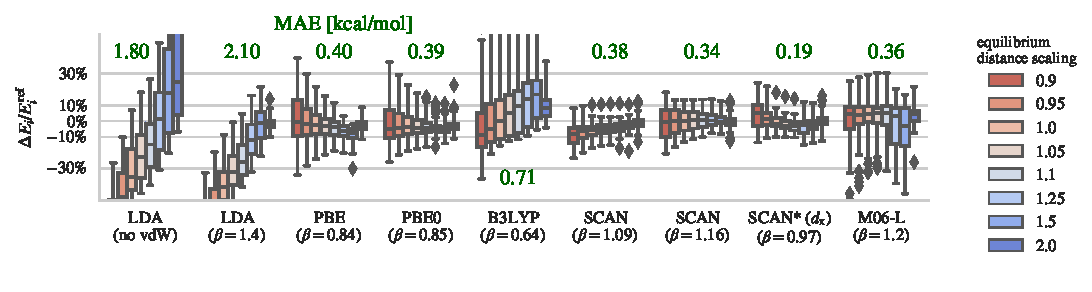
\includegraphics{../media/s66-dists}}
\caption{\textbf{Distributions of relative errors in binding energies on the S66 set of several DFT+MBD combinations.}
The distributions are displayed as box-and-whisker plots: a box shows the quartiles and whiskers represent the rest of the distribution, except for outliers that are more than 2.5-fold the interquartile distance from the box, which are shown individually.
The $x$-axis labels denote the functional and the value of the MBD range-separation parameter, $\beta^\text{MBD}$.
The blue--red spectrum encodes the scaling, $q$, of the respective equilibrium distances of individual complexes.
The green numbers indicate the mean absolute error (kcal/mol) for $q=1$.
The values of $\beta^\text{MBD}$ were selected as follows: $\beta$-values shown for PBE, PBE0, B3LYP, and M06 optimize both mean and standard deviation of relative errors (MRE, SDRE) around $q=1$; $\beta=1.4$ for LDA optimizes MRE and SDRE for $q=2$; and for SCAN and all $q$, $\beta=1.1$ optimizes SDRE, and $\beta=1.4$ optimizes MRE\@.
}\label{fig:s66-dists}
\end{figure*}

\paragraph{Van der Waals benchmark sets}

Whereas the vdW models have an explicit correlation range, the range of density functionals is only implicit, and the combined DFT+vdW models are therefore constructed by optimizing the range separation in vdW models against some benchmark properties, usually binding or lattice energies.
Several benchmark sets of vdW-bound systems have been established, of which we use predominantly three: the S66 set of 66 smaller organic dimers~\cite{RezacJCTC11}, the X23 set of 23 molecular crystals~\cite{ReillyJCP13}, and the S12L set of 12 large supramolecular complexes~\cite{RisthausJCTC13,AmbrosettiJPCL14}.
The S66 set is especially useful here, because each of the 66 dimers is given at 8 intermolecular distances distributed around the equilibrium distance.

The raw results of evaluating a method on a benchmark set consist of the distribution of errors, $E_i-E_i^\text{ref}$.
Since the interaction energies in vdW systems span orders of magnitude, we use relative errors, $\Delta_\mathrm rE_i=(E_i-E_i^\text{ref})/(-E_i^\text{ref})$ (assuming $E_i$ are negative).
The comparison of error distributions between different methods is simplified by introducing various statistical measures.
Two popular measures are the mean absolute error (MAE), $\sum_i\Delta_\mathrm rE_i/N$, and mean absolute relative error (MARE), $\sum_i\lvert\Delta_\mathrm rE_i\rvert/N$, which serve well as a single-number indicator of performance, but do not provide much insight into the actual error distributions.
Instead, we use the mean relative error (MRE), $\sum_i\Delta_\mathrm rE_i/N$, and the standard deviation of the relative errors (SDRE),
\[ \text{SDRE}=\frac1N\sqrt{\sum_i(\Delta_\mathrm rE_i-\text{MRE})^2} \]
This enables us to study both the systematic error of a method (overall underbinding or overbinding), represented by MRE, as well as the ``statistical'' error (how consistent a method is), represented by SDRE\@.

\section{Results}

\begin{figure*}
\makebox[\textwidth][c]{
\begin{tikzpicture}
\node[below right, anchor=base] at (0.5,-0.5) {\bfseries a};
\node[below right] at (0,0) {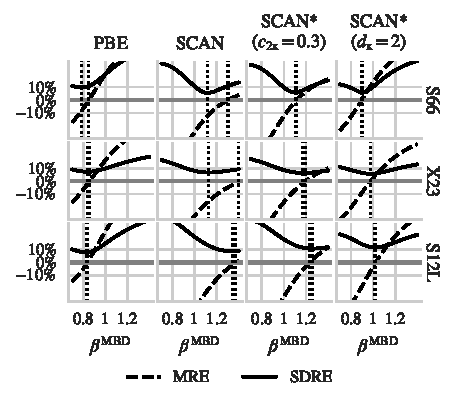
\includegraphics{../media/mbd-param-fitting.pdf}};
\node[below right, anchor=base] at (8.5,-0.5) {\bfseries b};
\node[below right] at (8.,-0.3) {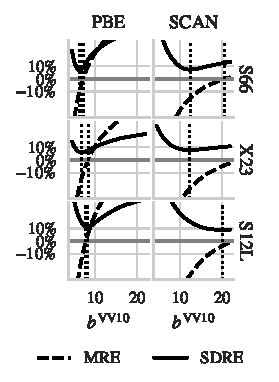
\includegraphics{../media/vv10-param-fitting.pdf}};
\node[below right, anchor=base] at (13.6,-0.5) {\bfseries c};
\node[below right] at (13.1,-0.3) {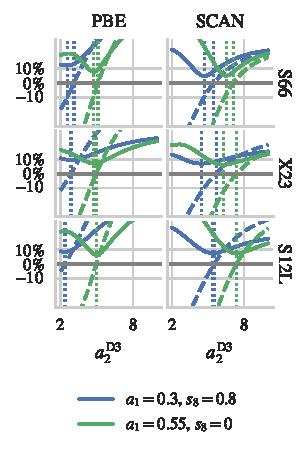
\includegraphics{../media/d3-param-fitting.pdf}};
\end{tikzpicture}
}
\caption{\textbf{Dependence of means (MRE) and standard deviations (SDRE) of relative errors in binding energies on range-separation parameters.}
Three long-range correlation models with their respective parameters are shown: (\textbf a) MBD with $\beta^\text{MBD}$, (\textbf b) VV10 with $b^\text{VV10}$, and (\textbf c) D3 with $a_2^\text{D3}$.
Density functionals correspond to columns, and benchmark sets to rows within each subplot.
SCAN* denotes two reparameterizations of the SCAN functional discussed in the text. % chktex 36
The vertical dotted lines show where MRE equals to zero or SDRE reaches minimum.
For DFT+D3, two choices are shown of the two other range-separation parameters in D3: $a_1^\text{D3}$ and $s_8^\text{D3}$.
}\label{fig:param-fitting}
\end{figure*}

To study the range of the density functionals LDA, PBE, PBE0, B3LYP, SCAN, SCAN0, and M06, we evaluated them, as well as the vdW methods MBD, VV10, and D3 at a range of their respective range-separation parameters, on the benchmark sets S66, X23, S12L, and other sets not discussed in this text.
We present a subset of these results below in Figures~\ref{fig:s66-dists} and~\ref{fig:param-fitting}, while the full data, obtained with FHI-aims~\cite{BlumCPC09} and Quantum Espresso~\cite{GiannozziJPCM09}, as well as computational details, are given in Supplementary Information.

On the case of the S66 set and different DFT+MBD combinations, Figure~\ref{fig:s66-dists} shows that summarizing the error distributions into a single number such as the mean absolute error reduces the method comparison to a one-dimensional classification, whereas comparing the full distributions in fact reveals distinct patterns specific to individual functionals.
Of the tested functionals, LDA is the only one that systematically overbinds S66 at equilibrium even without any long-range correction.
At the same time, when the equilibrium distances are scaled by 2, LDA predicts essentially no binding.
In this regard, although LDA binds vdW systems in equilibrium (too) strongly, it is very short-ranged.
The tail behavior can be fixed accurately by MBD with $\beta^\text{MBD}=1.4$, but of course nothing can be done about the short-range overbinding.
The increased overestimation of electron correlation with decreased distance then leads to the well-known underestimation of binding distances by LDA\@.
Already LDA thus illustrates that the degree to which a (semi-)local functional binds vdW systems is in general inconsequential for how well-suited it is for a combined DFT+vdW method. % chktex 36

In contrast, both PBE and PBE0 are strongly underbinding S66 on their own, but with MBD and appropriate range separation ($\beta^\text{MBD}\approx0.83$), the resulting PBE+MBD and PBE0+MBD methods are well balanced, with symmetric error distributions, MAE independent of distance, and SDRE monotonously increasing at shorter distances.
The admixture of exact exchange decreases SDRE from 10.2\% with PBE to 8.7\% with PBE0 at equilibrium, but in general has only a small effect.
Another hybrid GGA, B3LYP, behaves as a true opposite of LDA, being at the same time very repulsive, yet quite long-ranged.
Even with a fairly short-range correlation covered by MBD ($\beta^\text{MBD}\approx0.7$), B3LYP+MBD still underbinds at equilibrium, and perhaps more surprisingly at longer distances.
In contrast to PBE/PBE0, the distributions are highly asymmetric, with underbound outliers being mostly the hydrogen-bonded complexes.

With SCAN, optimizing for MRE and SDRE leads to different values of $\beta^\text{MBD}$, 1.4 and 1.1, respectively.
Both of these are substantially larger than that for PBE, demonstrating the longer range of SCAN\@.
When SDRE is optimized, SCAN+MBD overbinds by 10--15\% (MRE) for all distances, but SDRE is well balanced, and much better than that of PBE+MBD at short distances.
This should result in better predicted geometries.
When MRE is optimized, the profile of SCAN+MBD is similar to PBE+MBD, but with overall worse SDRE\@.
Adding exact exchange in SCAN0 (not shown) has even smaller effect than in PBE0, making the SCAN and SCAN0 error distributions almost indistinguishable.

Finally, M06 requires roughly the same amount of long-range correlation as SCAN, and most of the complexes from the S66 set are described well around equilibrium.
But several outliers are strongly overbound, and all complexes are overbound at longer distances, which is in line with previous studies~\cite{GoerigkJPCL15}.
Both issues may stem from the fact that the heavily fitted M06 is parametrized also on the S22 set, a smaller version of S66, but S66 contains additional complexes and out-of-equilibrium complexes for which M06 was not ``trained''.

Of the tested functionals, PBE and SCAN (or their hybrid versions) show a potential to work as general balanced DFT+vdW methods, but there is ambiguity in the range of the SCAN functional.
To rule out the possibility that this is simply an inability of MBD to adapt to a potentially more complex implicit range of SCAN with respect to PBE, we studied how MRE and SDRE of their combinations with MBD, VV10, and D3 depend on the respective range-separation parameters (Figure~\ref{fig:param-fitting}).
Comparing the results for the S66 set shows that the ambiguity in the range of SCAN is in fact universal across all vdW models, and not specific to MBD\@.
It is the case even for D3, which is potentially more flexible when adapting to a functional thanks to its three parameters.

Furthermore, Figure~\ref{fig:param-fitting} shows that whereas the optimal range separation of the vdW models is shared across different system types for the PBE functional, this is not the case for SCAN\@.
For SCAN, the discrepancy between MRE- and SDRE-optimizing range separation is even larger on the X23 set, but then it is reduced almost to zero for S12L.
Whereas the MRE-optimizing range separation is roughly constant across the benchmark sets, the SDRE-optimizing parameters differ substantially between S66 and X23 on one hand, and S12L on the other.
All these observations are true for all three vdW models.

\begin{figure}
\makebox[\linewidth][c]{
\begin{tikzpicture}
\node[below right] at (1.1,.1) {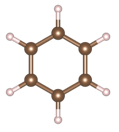
\includegraphics[height=1.2cm]{../media/bz2.png}};
\node[below right] at (2.2,.1) {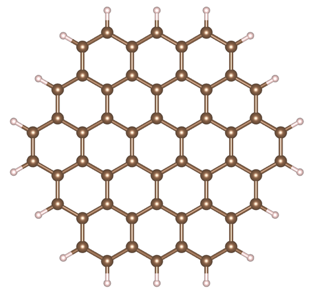
\includegraphics[height=1.2cm]{../media/cor21.png}};
\node[below right] at (3.5,.1) {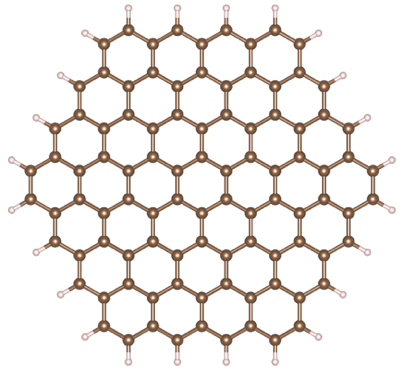
\includegraphics[height=1.2cm]{../media/cor22.png}};
\node[below right] at (6.7,0) {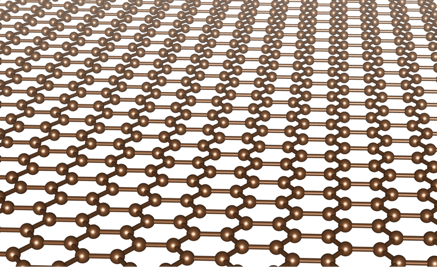
\includegraphics[height=1.0cm]{../media/gr2.png}};
\node[below right] at (0,-1) {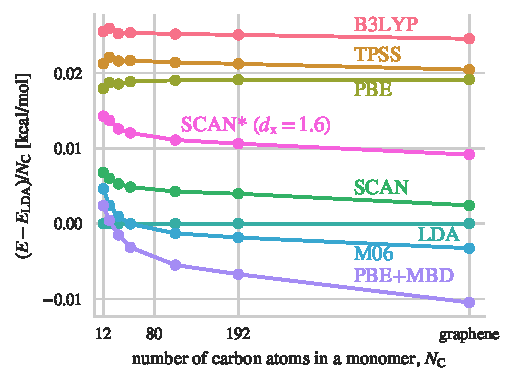
\includegraphics{../media/flakes.pdf}};
\end{tikzpicture}
}
\caption{\textbf{Binding energies of graphene-flake dimers.}
The individual data points correspond to (increasing in size) benzene, naphtalene, pyrene, coronene, two larger circular hexagonal flakes (shown), and graphene.
All dimers are in a parallel-displaced configuration, as cut out from a graphite crystal without any geometry relaxations.
The geometries and computational details are available in Supplementary Information.
The plotted quantity is binding energy with respect to the LDA binding energy, per carbon atom.
The (infinite) number of atoms in graphene is set arbitrarily to 500.
}\label{fig:flakes}
\end{figure}

To gain further insight into the range of the functionals beyond statistical analysis, we calculated the binding energies of a series of graphene-flake dimers dimers ranging from a benzene dimer to a graphene bilayer using DFT without any long-range correction (Figure~\ref{fig:flakes}).
We consider LDA as a reference short-range functional, accounting for any potential edge effects, and PBE+MBD as a reference full-range method.
The functionals B3LYP, PBE, and TPSS have a similar behavior to LDA, with the binding energies being offset only by a constant.
In contrast, the SCAN and M06 show a much stronger dependence on the system size, both at the small and large ends of the spectrum.
The difference in the offset to LDA between benzene dimer and graphene is 60\% for M06 and 35\% for SCAN with respect to PBE+MBD\@.
The ability to capture at least partially this system-size effect could be seen as advantageous, but it is unfortunate for developing DFT+vdW methods, because it breaks the core assumption that the functionals behave as short-range models of the electron correlation.
After all, these functionals are semi-local by construction and the fact that they are sensitive to this strongly nonlocal environment is contradicting this semi-locality.

Both SCAN and M06 are meta-GGAs, but so is TPSS, which does not show this sensitivity.
We speculate, and partially substantiate this speculation, that in case of SCAN, this sensitivity is caused by the particular parametrization of its dependence on the dimensionless electron localization parameter, $\alpha$ (see Background).
The values of $\alpha$ typically count in single figures within the electronic valence shells and decay slowly to zero with distance from the electronic system, while crossing $\alpha=1$ at some point~\cite{SunPRL13,BeckeJCP90}.
Among meta-GGA functionals, SCAN has a relatively wide plateau around $\alpha=1$ (due to Eq.~\ref{eq:scan-interp})~\cite{LoosJCP17}, where the enhancement factor, $F_\mathrm x$, is equal to 1, the value for the uniform electron gas.
This results in spatial regions in the electron density tails (dominated by HOMO, the highest-occupied molecular orbital) that are described with a uniform-like functional instead of the more appropriate single-orbital form of $\alpha\approx0$.
This can lead to sudden spikes in the exchange-correlation potential fairly outside the spatial regions where covalent bonding occurs~\cite{Gerit-private}.

\begin{figure}
\centering
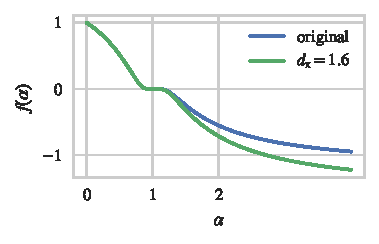
\includegraphics{../media/scan-interp}
\caption{\textbf{Interpolation and extrapolation used in the SCAN exchange functional.}
The fixed points that are inter- and extrapolated are $\alpha=0$ and $\alpha=1$.
The shape of the function is controlled with three parameters, $c_\mathrm{1x}=0.667$, $c_\mathrm{2x}=0.8$, and $d_\mathrm x=1.24$ (original values).
}\label{fig:scan-interp}
\end{figure}

In the series of graphene-flake dimers, the electronic gap (calculated with SCAN) decreases from 4.7\,eV for benzene dimer to 0.9\,eV for graphene bilayer, which makes the density tail decay slower with increasing system size.
Because the $\alpha=1$ behavior of SCAN makes it quite sensitive in the density tails, whose overlap also encodes the vdW bonding on the electron-density level, it only makes sense that SCAN is able to extract the nonlocal information about the system size via the decreasing electronic gap.
This mechanism could be also partially responsible for the discrepancies in optimal range separation for SCAN observed on the S66, X23, and S12L sets.

To check this hypothesis, we constructed two reparameterizations of SCAN and tested them on these benchmark sets.
We focused on the three parameters in Eq.~\ref{eq:scan-interp} because their values are determined weakly, having been fitted only to system-specific rather than universal norms.
We found that either changing $c_\mathrm{2x}$ from 0.8 to 0.3 or changing $d_\mathrm x$ from 1.24 to 2 (Figure~\ref{fig:scan-interp}) substantially improves the consistency of SCAN in describing vdW systems (Figure~\ref{fig:param-fitting}a), by removing the ambiguity in whether to optimize for MRE or SDRE\@.
The overall performance is also improved, bringing MARE of SCAN*+MBD on S66 to only 4.5\% in both cases, a two-fold improvement over PBE+MBD\@.
Both reparameterizations change behavior of the functional in the regions of overlap of closed shells, making the slopes of the interpolating function more similar on both sides of $\alpha=1$.
This is in line with the hypothesis that it is the behavior around $\alpha=1$ (uniform-gas limit) that is causing the imbalanced behavior for vdW systems.
The $c_\mathrm{2x}$-variant retains the longer range of SCAN (optimal $\beta^\text{MBD}$ of 1.1 on S66), while the $d_\mathrm x$-variant brings it closer to that of PBE ($\beta^\text{MBD}$ of 0.9).
However, both reparameterizations still suffer from dependence of the optimal range separation on system type (cf.\ PBE), with optimal $\beta^\text{MBD}$ for X23 and S12L being larger by 0.1 than for S66.

\section{Discussion}

SCAN has been previously combined with VV10 by \citet{PengPRX16} and with D3 and VV10 by \citet{BrandenburgPRB16}.
The obtained optimal values of $b^\text{VV10}$ were 15.7 and 14.0, respectively, and optimal parametrization of D3 was found to be $s_8^\text{D3}=0$, $a_1^\text{D3}=0.54$ and $a_2^\text{D3}=5.4$.
From Figure~\ref{fig:param-fitting}, this corresponds to a compromise between the systematic (MRE) and statistical (SDRE) error for SCAN+VV10, and to optimal statistical error for SCAN+D3, in all cases leading to some degree of systematic overbinding.
\citet{BrandenburgPRB16} associated this tendency mainly with hydrogen-bonded systems, which is in line with the observed overbinding of various ice structures by SCAN (without any vdW correction)~\cite{ChenPRB16}.

\citet{PengPRX16} argued that shifting the range separation between a semi-local functional and a vdW model towards the latter is beneficial.
Such a shift could also avoid some of the problems that long-range correlation models need to deal with at short range, such as the quadrupole interaction.
Our results confirm that such a shift is indeed possible in principle, but with the caveat that the description of the intermediate range by the density functional must be balanced and independent of system size.

The two reparameterizations of the SCAN functional illustrate that the behavior of the range of even a very sophisticated functional can be changed by a single parameter, whose value is not fixed by any hard constraint.
We did not evaluate any other properties besides vdW binding, and it is quite possible that the new parameter values would introduce regressions for other systems.
To give a true alternative parametrization, the original fitting procedure would need to be performed with an additional constraint on vdW binding, perhaps expressed via a single simple system, which is beyond the scope of this work.
However, the restored smoothness of the slope of the interpolating function around $\alpha=1$ suggests that there is a solid physical motivation behind these reparameterizations.

\section{Conclusions}

We showed that although the range of semi-local functionals cannot be known explicitly, it is still possible to obtain meaningful and detailed information about their range by probing them with long-range correlation models, for which the range is known explicitly.
This information can be then used to construct the functionals in such a way that their range is consistent across different systems, a condition necessary for a generally applicable DFT+vdW method.
After all, semi-local functionals and vdW methods model two interconnected parts of a single thing, the electron correlation, and it makes only sense to develop them in tandem.


\subsection{Acknowledgements}

A.T.\ acknowledges support from the European Research Council (ERC), Consolidator Grant BeStMo.

\subsection{Supporting Information}

Computational details, detailed description of the computational protocol, references to raw data used to generate the figures in the manuscript; calculations on the 3B-69 set for 3-body interactions, rare-gas dimers, and the X40 set; plot of the dependence of the errors on system size; extensions of some figures from the main text to more functionals; geometries of all structures used in the manuscript.

This information is available free of charge via the Internet at http://pubs.acs.org.

\begingroup
\setlength\bibsep{0pt}
\footnotesize
\bibliography{refs-zotero,refs}
\endgroup

\end{document}
